%==============================================================================
% PD5 - A Pipelined RV32I RISC-V Core with Forwarding, Stall, and Flush Logic
% Technical Documentation
%
% Build:  pdflatex main.tex   (run twice for TOC / cross-references)
%    or:  latexmk -pdf main.tex
% Dependencies: a standard TeX distribution with TikZ (MiKTeX / TeX Live).
%               No bibtex pass required (inline thebibliography).
%==============================================================================
\documentclass[11pt,a4paper]{article}

\usepackage[T1]{fontenc}
\usepackage[utf8]{inputenc}
\usepackage{lmodern}
\usepackage[margin=1in]{geometry}
\usepackage{amsmath}
\usepackage{graphicx}
\usepackage{xcolor}
\usepackage{booktabs}
\usepackage{longtable}
\usepackage{array}
\usepackage{caption}
\usepackage{enumitem}
\usepackage{tikz}
\usetikzlibrary{positioning,arrows.meta,calc,fit,backgrounds,shapes.geometric}
\usepackage[colorlinks=true,linkcolor=blue!55!black,urlcolor=blue!55!black,
            citecolor=blue!55!black]{hyperref}

% --- convenience macros ------------------------------------------------------
\newcommand{\code}[1]{\texttt{#1}}          % monospace signal / file names
\newcommand{\sig}[1]{\texttt{#1}}
\newcommand{\hex}[1]{\texttt{0x#1}}

% --- colours for TikZ diagrams ----------------------------------------------
\definecolor{stagefill}{RGB}{223,237,248}
\definecolor{stageline}{RGB}{ 41,128,185}
\definecolor{regfill}{RGB}{252,243,207}
\definecolor{regline}{RGB}{183,149, 11}
\definecolor{auxfill}{RGB}{234,242,225}
\definecolor{auxline}{RGB}{ 88,133, 39}
\definecolor{hazfill}{RGB}{250,229,229}
\definecolor{hazline}{RGB}{176, 58, 46}
\definecolor{fwdarrow}{RGB}{176, 58, 46}

\captionsetup{font=small,labelfont=bf}

%==============================================================================
\begin{document}

%------------------------------------------------------------------ Title page
\begin{titlepage}
\centering
\vspace*{2.2cm}

{\Large\scshape York University\par}
{\large EECS 4201 --- Computer Architecture and Organization\par}
\vspace{2.4cm}

\rule{\linewidth}{0.4pt}\\[0.5cm]
{\huge\bfseries PD5: A Pipelined RV32I RISC-V Core\\[0.35cm]
with Forwarding, Stall, and Flush Logic\par}
\vspace{0.5cm}
\rule{\linewidth}{0.4pt}\\[0.8cm]

{\large Technical Documentation of the Final Project Deliverable\par}
\vspace{2.6cm}

{\large\textbf{Author:} Salwan Aldhahab\par}
\vspace{0.4cm}
{\large\textbf{Hardware Description Language:} SystemVerilog\par}
{\large\textbf{Target ISA:} RV32I (32-bit base integer)\par}
{\large\textbf{Verification:} ModelSim (Intel FPGA / Quartus) $\cdot$ \code{rv32-bmarks}\par}

\vfill
{\large July 2026\par}
\end{titlepage}

%--------------------------------------------------------------------- Abstract
\begin{abstract}
\noindent
This document describes the design and verification of \textbf{PD5}, the final and
complete deliverable of a multi-stage RISC-V processor project. PD5 implements a
fully-pipelined, five-stage, in-order RISC-V core that supports the RV32I base integer
instruction set, written entirely in SystemVerilog. The core is organised into the
classic \emph{Instruction Fetch}, \emph{Instruction Decode}, \emph{Execute},
\emph{Memory}, and \emph{Writeback} stages, separated by four pipeline registers. To
sustain one-instruction-per-cycle throughput while preserving program correctness, the
design integrates a dedicated hazard unit that performs \emph{data forwarding}
(EX/MEM~$\rightarrow$~EX and MEM/WB~$\rightarrow$~EX bypassing), \emph{stalling} for
load--use and write-to-decode dependencies, and \emph{flushing} of speculatively fetched
instructions following taken branches and jumps. The core was compiled and simulated with
ModelSim (Intel FPGA Starter Edition, part of the Intel Quartus toolchain), driven from a
bash/GNU~Make flow, and debugged through VCD waveform inspection. It was validated against
directed pattern tests, thirteen targeted pipeline micro-tests, and the project
\code{rv32-bmarks} benchmark suite --- comprising thirty-eight RV32UI instruction-level
tests and ten full C-language benchmarks --- \textbf{all of which pass}.
\end{abstract}

\tableofcontents
\newpage

%==============================================================================
\section{Introduction}
%==============================================================================
The overall course project incrementally constructs a RISC-V processor across a sequence
of \emph{Project Deliverables} (PD0 through PD5). Each deliverable adds one conceptual
layer: PD0 establishes the toolchain and a small three-stage warm-up pipeline; PD1--PD2
build the memory subsystem, instruction fetch, decode, and control; PD3 adds the execute
stage, ALU, and branch comparison logic; and PD4 assembles these into a functionally
complete \emph{single-cycle} datapath together with the register file.

\textbf{PD5 is the culmination of this progression.} It reuses the datapath building
blocks proven in the earlier deliverables and transforms the single-cycle machine into a
genuine five-stage pipeline. The essential new engineering content of PD5 is therefore not
the arithmetic or the decoding --- those are inherited --- but the machinery required to
make a pipeline behave correctly in the presence of \emph{hazards}: the pipeline registers
that decouple the stages, the forwarding network that resolves most data dependencies
without penalty, the stall logic that handles the dependencies forwarding cannot cover,
and the flush logic that discards wrongly fetched instructions after control-flow changes.

This report documents PD5 exclusively. Earlier deliverables are referenced only as
lineage. Section~\ref{sec:background} reviews the RV32I subset and the pipeline hazard
taxonomy. Section~\ref{sec:arch} presents the top-level architecture.
Section~\ref{sec:datapath} details each datapath module. Section~\ref{sec:pipelinereg}
covers the pipeline registers, and Section~\ref{sec:hazard} --- the heart of PD5 ---
covers hazard handling. Section~\ref{sec:verif} describes the verification methodology and
toolchain, Section~\ref{sec:results} reports results, and Section~\ref{sec:conclusion}
concludes. Appendices list the module inventory, the debug probe signals, and the full
benchmark set.

%==============================================================================
\section{Background}
\label{sec:background}
%==============================================================================
\subsection{The RV32I instruction set}
RV32I is the 32-bit base integer instruction set of the RISC-V architecture. It defines
thirty-two 32-bit general-purpose registers (\sig{x0}--\sig{x31}), with \sig{x0} hardwired
to zero, and a program counter. Instructions are a fixed 32 bits wide and fall into six
encoding formats distinguished by how their immediate operand is assembled from the
instruction word. Table~\ref{tab:formats} summarises these formats and the instruction
classes PD5 implements.

\begin{table}[h]
\centering
\caption{RV32I instruction formats and the operations supported by PD5.}
\label{tab:formats}
\small
\begin{tabular}{@{}c l l@{}}
\toprule
\textbf{Format} & \textbf{Representative instructions} & \textbf{Immediate assembled from} \\
\midrule
R & \sig{add sub and or xor sll srl sra slt sltu} & (none; register--register) \\
I & \sig{addi andi ori xori slli srli srai slti}   & sign-extended \sig{insn[31:20]} \\
  & \sig{sltiu}, loads (\sig{lb lh lw lbu lhu}), \sig{jalr} & \\
S & stores (\sig{sb sh sw})                          & \sig{insn[31:25]}, \sig{insn[11:7]} \\
B & branches (\sig{beq bne blt bge bltu bgeu})       & \sig{insn[31]}, \sig{insn[7]}, \sig{insn[30:25]}, \sig{insn[11:8]} \\
U & \sig{lui}, \sig{auipc}                            & \sig{insn[31:12]} in bits 31:12 \\
J & \sig{jal}                                         & \sig{insn[31]}, \sig{insn[19:12]}, \sig{insn[20]}, \sig{insn[30:21]} \\
\bottomrule
\end{tabular}
\end{table}

\subsection{The five-stage pipeline and hazards}
A pipelined processor overlaps the execution of consecutive instructions, ideally
completing one instruction per clock cycle. The classic five-stage organisation splits
instruction processing into Instruction Fetch (IF), Instruction Decode / register read
(ID), Execute / address calculation (EX), Memory access (MEM), and register Writeback
(WB). Because up to five instructions are then ``in flight'' simultaneously, three classes
of \emph{hazard} can corrupt results unless handled:

\begin{description}[leftmargin=1.6cm,style=nextline]
  \item[Structural hazards] two instructions competing for the same hardware resource in
    the same cycle. PD5 avoids these by using \emph{separate} instruction and data memory
    ports and a register file that writes and reads in the same cycle.
  \item[Data hazards] an instruction needing a result that an earlier, not-yet-retired
    instruction has produced. PD5 resolves most of these by \emph{forwarding} and the
    remainder by \emph{stalling} (Section~\ref{sec:hazard}).
  \item[Control hazards] the next instruction address being unknown until a branch or jump
    resolves. PD5 fetches sequentially by default and \emph{flushes} the wrongly fetched
    instructions when a branch is taken or a jump executes.
\end{description}

%==============================================================================
\section{Architecture Overview}
\label{sec:arch}
%==============================================================================
The top-level module \code{pd5} instantiates every stage, the two memory instances, the
register file, the four pipeline registers, and the hazard unit, and wires them together
with the forwarding multiplexers. Figure~\ref{fig:datapath} shows the overall structure.

\begin{figure}[h]
\centering
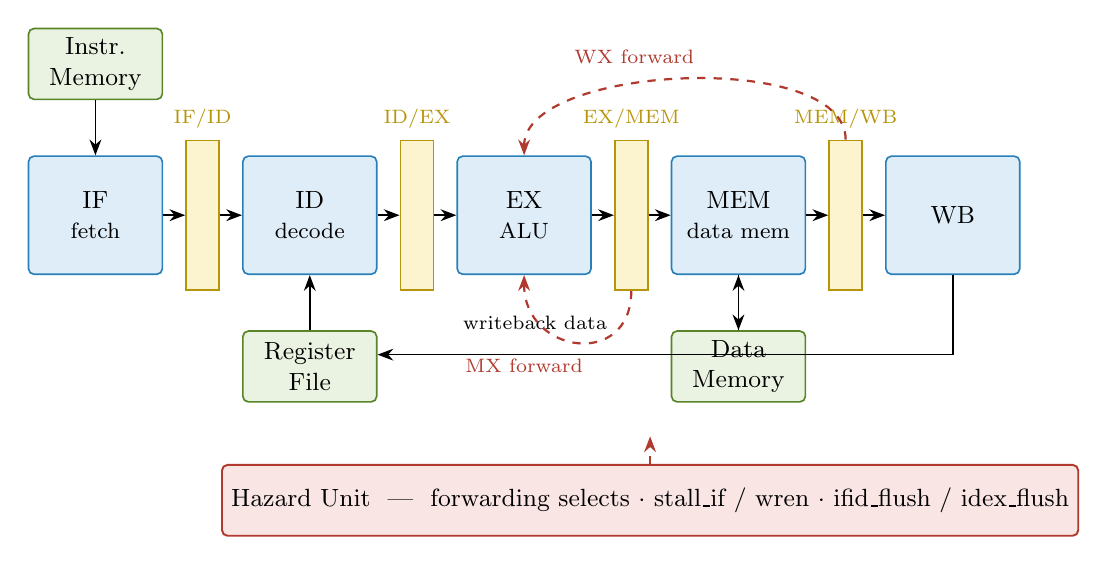
\begin{tikzpicture}[
    font=\small,
    stage/.style={draw=stageline,fill=stagefill,line width=0.6pt,rounded corners=2pt,
                  minimum width=1.7cm,minimum height=1.5cm,align=center},
    preg/.style={draw=regline,fill=regfill,line width=0.6pt,
                 minimum width=0.42cm,minimum height=1.9cm},
    aux/.style={draw=auxline,fill=auxfill,line width=0.6pt,rounded corners=2pt,
                minimum width=1.7cm,minimum height=0.9cm,align=center},
    haz/.style={draw=hazline,fill=hazfill,line width=0.7pt,rounded corners=2pt,
                minimum width=10.5cm,minimum height=0.9cm,align=center},
    flow/.style={-{Stealth[length=2mm]},line width=0.6pt},
    fwd/.style={-{Stealth[length=2mm]},draw=fwdarrow,line width=0.8pt,dashed},
]
% --- stage row ---
\node[stage] (if)  at (0,0)      {IF\\\footnotesize fetch};
\node[preg,right=0.28cm of if]  (r1) {};
\node[stage,right=0.28cm of r1] (id) {ID\\\footnotesize decode};
\node[preg,right=0.28cm of id]  (r2) {};
\node[stage,right=0.28cm of r2] (ex) {EX\\\footnotesize ALU};
\node[preg,right=0.28cm of ex]  (r3) {};
\node[stage,right=0.28cm of r3] (me) {MEM\\\footnotesize data mem};
\node[preg,right=0.28cm of me]  (r4) {};
\node[stage,right=0.28cm of r4] (wb) {WB};

% pipeline register labels
\node[above=0.02cm of r1,font=\scriptsize,text=regline] {IF/ID};
\node[above=0.02cm of r2,font=\scriptsize,text=regline] {ID/EX};
\node[above=0.02cm of r3,font=\scriptsize,text=regline] {EX/MEM};
\node[above=0.02cm of r4,font=\scriptsize,text=regline] {MEM/WB};

% aux blocks
\node[aux,above=0.7cm of if] (imem) {Instr.\\Memory};
\node[aux,below=0.7cm of id] (rf)   {Register\\File};
\node[aux,below=0.7cm of me] (dmem) {Data\\Memory};

% straight dataflow
\draw[flow] (if) -- (r1);
\draw[flow] (r1) -- (id);
\draw[flow] (id) -- (r2);
\draw[flow] (r2) -- (ex);
\draw[flow] (ex) -- (r3);
\draw[flow] (r3) -- (me);
\draw[flow] (me) -- (r4);
\draw[flow] (r4) -- (wb);

\draw[flow] (imem) -- (if);
\draw[flow] (rf.north) -- (id.south);
\draw[flow] (me) -- (dmem);
\draw[flow] (dmem) -- (me);

% writeback path back to register file
\draw[flow] (wb.south) |- ($(rf.east)+(0,0.15)$);
\node[font=\scriptsize] at ($(rf.east)+(2.0,0.55)$) {writeback data};

% forwarding arrows (EX/MEM and MEM/WB back into EX)
\draw[fwd] (r3.south) .. controls +(0,-1.0) and +(0,-1.0) .. (ex.south);
\draw[fwd] (r4.north) .. controls +(0,1.15) and +(0,1.15) .. (ex.north);
\node[text=fwdarrow,font=\scriptsize] at ($(ex.south)+(0.0,-1.15)$) {MX forward};
\node[text=fwdarrow,font=\scriptsize] at ($(ex.north)+(1.4,1.25)$) {WX forward};

% hazard unit spanning the datapath
\node[haz] (hz) at ($(rf)!0.5!(dmem)+(1.6,-1.7)$) {Hazard Unit\ \ ---\ \
   forwarding selects $\cdot$ stall\_if / wren $\cdot$ ifid\_flush / idex\_flush};
\draw[fwd] (hz.north) -- ++(0,0.35);
\end{tikzpicture}
\caption{PD5 five-stage datapath. Solid arrows are the normal per-cycle dataflow; dashed
red arrows are the forwarding paths from the EX/MEM (MX) and MEM/WB (WX) pipeline
registers back into the Execute stage. The hazard unit observes register indices across
the pipeline and drives the forwarding, stall, and flush controls.}
\label{fig:datapath}
\end{figure}

\subsection{Stage summary}
Table~\ref{tab:stages} lists each stage, its principal module(s), and its responsibility.

\begin{table}[h]
\centering
\caption{Pipeline stages and their implementing modules.}
\label{tab:stages}
\small
\begin{tabular}{@{}l l l@{}}
\toprule
\textbf{Stage} & \textbf{Module(s)} & \textbf{Responsibility} \\
\midrule
IF  & \code{fetch}, \code{memory} (imem) & Hold/advance PC; read instruction word. \\
ID  & \code{decode}, \code{igen}, \code{control}, \code{register\_file}
    & Extract fields; build immediate; generate control; read \sig{rs1}/\sig{rs2}. \\
EX  & \code{alu} (in \code{execute}), \code{branch\_control}
    & Arithmetic/logic; address calc; branch decision. \\
MEM & \code{memory} (dmem) & Load/store data memory access. \\
WB  & \code{writeback} & Select ALU / memory / PC+4 result to write back. \\
\bottomrule
\end{tabular}
\end{table}

\subsection{Memory map and register conventions}
The core uses a flat, byte-addressable memory of \code{MEM\_DEPTH} = \code{1048576} bytes
(1~MiB). Program images are loaded as 32-bit words and unpacked little-endian into the
byte array. Both the instruction and data memories are parameterised with a base address
of \hex{01000000}; addresses at or above the base are mapped into the memory window and
wrapped modulo its size. On reset the register file clears all registers and initialises
the stack pointer \sig{x2} to \hex{01100000}, placing the stack 1~MiB above the program
base. Register \sig{x0} is permanently forced to zero on every clock edge, regardless of
any write.

%==============================================================================
\section{Datapath Implementation}
\label{sec:datapath}
%==============================================================================
This section describes each datapath module in program order. For every module a short
behavioural description is followed by a table of its interface signals.

\subsection{Fetch and instruction memory}
The \code{fetch} module holds the program counter in a reset-initialised register (reset
value \hex{01000000}). On each clock edge it either loads a supplied target address or
advances by four. The next-address decision is made at the top level: while the pipeline
stalls, the PC is held at its current value; when the Execute stage signals a taken branch
or a jump, the PC loads the computed target; otherwise it advances sequentially. The
instruction word itself comes from a dedicated \code{memory} instance configured as
read-only instruction memory, addressed by the current PC.

\begin{table}[h]
\centering
\caption{\code{fetch} interface.}
\label{tab:fetch}
\small
\begin{tabular}{@{}l l l@{}}
\toprule
\textbf{Signal} & \textbf{Dir.} & \textbf{Description} \\
\midrule
\sig{clk}, \sig{rst}     & in  & Clock and reset. \\
\sig{pcsel\_i}           & in  & Select target (\sig{1}) vs.\ sequential PC+4 (\sig{0}). \\
\sig{pctarget\_i}        & in  & Branch/jump target address to load. \\
\sig{pc\_o}              & out & Current program counter. \\
\bottomrule
\end{tabular}
\end{table}

\subsection{Decode, immediate generation, and control}
The \code{decode} module splits the fetched word into its architectural fields ---
\sig{opcode}, \sig{rd}, \sig{rs1}, \sig{rs2}, \sig{funct3}, \sig{funct7}, and a shift
amount --- selecting the correct fields per instruction format. It instantiates the
\code{igen} immediate generator, which assembles the sign-extended immediate for the I,
S, B, U, and J formats according to Table~\ref{tab:formats}.

The \code{control} module is a purely combinational decoder that maps the opcode (and,
where needed, \sig{funct3}/\sig{funct7}) onto the datapath control lines. Its outputs are
summarised in Table~\ref{tab:control}. It emits safe defaults (no register write, no
memory access) so that unrecognised opcodes are inert.

\begin{table}[h]
\centering
\caption{Control signals produced by the \code{control} decoder per opcode class.}
\label{tab:control}
\small
\begin{tabular}{@{}l c c c c c l@{}}
\toprule
\textbf{Class} & \sig{regwren} & \sig{memren} & \sig{memwren} & \sig{pcsel} & \sig{wbsel} & \textbf{ALU op} \\
\midrule
R-type   & 1 & 0 & 0 & 0 & 00 (ALU) & by \sig{funct3}/\sig{funct7} \\
I-type   & 1 & 0 & 0 & 0 & 00 (ALU) & by \sig{funct3} \\
Load     & 1 & 1 & 0 & 0 & 01 (mem) & ADD (address) \\
Store    & 0 & 0 & 1 & 0 & 00       & ADD (address) \\
Branch   & 0 & 0 & 0 & 0 & 00       & SUB (compare) \\
\sig{jal}  & 1 & 0 & 0 & 1 & 10 (PC+4) & ADD (target) \\
\sig{jalr} & 1 & 0 & 0 & 1 & 10 (PC+4) & ADD (target) \\
\sig{lui}  & 1 & 0 & 0 & 0 & 00       & pass immediate \\
\sig{auipc}& 1 & 0 & 0 & 0 & 00       & PC + immediate \\
\bottomrule
\end{tabular}
\end{table}

\subsection{Register file}
The \code{register\_file} provides two asynchronous (combinational) read ports and one
synchronous write port. Reads occur in the Decode stage; writes are committed on the
rising clock edge from the Writeback stage. Reads of \sig{x0} return zero, and writes to
\sig{x0} are suppressed, so the zero register is invariant. Because the write is
synchronous and the reads are combinational, a value written on a clock edge is visible to
a read in the \emph{same} cycle only through forwarding or a stall --- a subtlety handled
by the hazard unit (Section~\ref{sec:hazard}).

\subsection{Execute: ALU and branch control}
The Execute stage centres on the \code{alu} module (in \code{execute.sv}). Driven by the
opcode and function fields, it performs the full RV32I arithmetic, logical, shift, and
comparison repertoire; computes effective addresses for loads and stores (\sig{rs1} +
immediate); computes branch and \sig{jal} targets (PC + immediate) and the \sig{jalr}
target (\sig{rs1} + immediate); and passes the immediate through for \sig{lui}. The
supported ALU operations are listed in Table~\ref{tab:alu}.

Branch conditions are resolved by the \code{branch\_control} submodule, which produces an
``equal'' flag and a ``less-than'' flag (signed or unsigned per \sig{funct3}). The ALU
combines these into the final branch-taken decision for each branch type (for example,
\sig{bge} is taken when not-less-than or equal). The \sig{brtaken} output steers the PC in
Fetch.

\begin{table}[h]
\centering
\caption{ALU operations implemented in the Execute stage.}
\label{tab:alu}
\small
\begin{tabular}{@{}l l@{\hspace{2cm}} l l@{}}
\toprule
\textbf{Op} & \textbf{Function} & \textbf{Op} & \textbf{Function} \\
\midrule
ADD  & \sig{rs1 + rs2/imm}          & SRL  & logical right shift \\
SUB  & \sig{rs1 - rs2}              & SRA  & arithmetic right shift \\
AND  & bitwise AND                  & SLT  & set-less-than (signed) \\
OR   & bitwise OR                   & SLTU & set-less-than (unsigned) \\
XOR  & bitwise XOR                  & LUI  & pass immediate \\
SLL  & logical left shift           & AUIPC& \sig{pc + imm} \\
\bottomrule
\end{tabular}
\end{table}

\subsection{Memory}
The \code{memory} module is byte-addressable and supports byte, halfword, and word
accesses selected by \sig{funct3}. Reads are combinational and apply sign- or zero-
extension (\sig{lb}/\sig{lh} sign-extend; \sig{lbu}/\sig{lhu} zero-extend; \sig{lw} loads
a full word). Writes are synchronous and size-aware (\sig{sb}/\sig{sh}/\sig{sw}); writes
to address zero are ignored. The same module type serves as both the read-only instruction
memory in Fetch and the read/write data memory in the Memory stage.

\subsection{Writeback}
The \code{writeback} module selects, via the two-bit \sig{wbsel}, which value is committed
to the register file: the ALU result (\sig{00}), data loaded from memory (\sig{01}), or
the return address PC+4 for jumps (\sig{10}). A second instance of this module is used at
the top level purely to compute the branch/jump target address that feeds the Fetch stage,
keeping the next-PC calculation and the register-writeback selection in one reusable block.

%==============================================================================
\section{Pipeline Registers}
\label{sec:pipelinereg}
%==============================================================================
All four inter-stage registers live in a single \code{pipeline\_registers} module: IF/ID,
ID/EX, EX/MEM, and MEM/WB. Each register latches, on the rising clock edge, the data and
control signals its downstream stage requires (Table~\ref{tab:pregs}). Every register
supports \emph{stalling} through a write-enable input and \emph{reset} to a defined idle
state; the two front-end registers (IF/ID and ID/EX) additionally support \emph{flushing}.

A flush inserts a \emph{bubble} --- a benign no-operation --- into the pipeline. In the
IF/ID register a flush loads the canonical NOP encoding \hex{00000013} (\sig{addi x0, x0,
0}) in place of the fetched instruction, so the squashed instruction decodes to something
harmless. In the ID/EX register a flush clears the memory and branch control signals so
the bubbled instruction performs no memory access and cannot alter control flow. This
mechanism is what allows the hazard unit to cancel instructions cheaply after a taken
branch or during a stall.

\begin{table}[h]
\centering
\caption{Principal contents carried by each pipeline register.}
\label{tab:pregs}
\small
\begin{tabular}{@{}l l@{}}
\toprule
\textbf{Register} & \textbf{Carries (selected)} \\
\midrule
IF/ID  & PC, fetched instruction word. \\
ID/EX  & PC, \sig{rs1}/\sig{rs2} data and indices, \sig{rd}, immediate, \sig{funct3}/\sig{funct7}, \\
       & opcode, and all control signals (\sig{regwren}, \sig{memren}, \sig{memwren}, \sig{wbsel}, \sig{alusel}, \sig{pcsel}). \\
EX/MEM & PC, ALU result, store data and \sig{rs2} index, \sig{rd}, \sig{funct3}, \\
       & \sig{regwren}/\sig{memren}/\sig{memwren}/\sig{wbsel}, branch-taken flag. \\
MEM/WB & PC, ALU result, loaded memory data, \sig{rd}, \sig{regwren}, \sig{wbsel}. \\
\bottomrule
\end{tabular}
\end{table}

Note that the EX/MEM register additionally forwards the \sig{rs2} \emph{index} into the
Memory stage. This is not needed for ordinary datapath function but supports store-data
forwarding (the WM case in Section~\ref{sec:hazard}).

%==============================================================================
\section{Hazard Handling}
\label{sec:hazard}
%==============================================================================
The hazard unit is the defining contribution of PD5. It observes the register indices and
control signals present in the ID, EX, MEM, and WB stages and drives three families of
control output: forwarding selects, stall/write-enable signals, and flush signals.
Table~\ref{tab:hazards} summarises every case; the subsections that follow explain each.

\begin{table}[h]
\centering
\caption{Hazard detection conditions and the resulting pipeline action.}
\label{tab:hazards}
\small
\begin{tabular}{@{}l p{6.6cm} l@{}}
\toprule
\textbf{Hazard} & \textbf{Detection condition} & \textbf{Action} \\
\midrule
Forward MX (rs1/rs2) & MEM stage writes a register (\sig{$\neq$ x0}) that an EX operand needs & Bypass EX/MEM ALU result into EX \\
Forward WX (rs1/rs2) & WB stage writes a register (\sig{$\neq$ x0}) that an EX operand needs (and no MX match) & Bypass MEM/WB data into EX \\
Load--use & EX holds a load whose \sig{rd} matches an ID source register & Stall 1 cycle + bubble \\
Write--decode (WD) & WB writes a register that an ID source needs & Stall 1 cycle + bubble \\
Control (branch/jump) & EX signals branch-taken, or EX opcode is \sig{jal}/\sig{jalr} & Flush IF/ID and ID/EX \\
Store forward (WM) & MEM holds a store whose source \sig{rs2} equals the WB destination & Substitute WB data as store data \\
\bottomrule
\end{tabular}
\end{table}

\subsection{Data forwarding}
Most data dependencies are resolved without any stall by \emph{forwarding} (bypassing) a
result from a later pipeline stage directly into the Execute stage, before it has been
written back to the register file. PD5 implements two forwarding paths for each source
operand:

\begin{itemize}[leftmargin=1.4cm]
  \item \textbf{MX forwarding} --- the ALU result waiting in the EX/MEM register is routed
    back into EX. This covers a dependency on the immediately preceding instruction.
  \item \textbf{WX forwarding} --- the value in the MEM/WB register (ALU result or loaded
    data, already writeback-selected) is routed back into EX. This covers a dependency on
    the instruction two ahead.
\end{itemize}

The hazard unit produces a two-bit select for each operand, encoded as in
Table~\ref{tab:fwdsel}. MX takes priority over WX so that the most recent producer wins.
Crucially, the forwarded operands feed \emph{both} the ALU and the branch comparator, so
branches that depend on a just-computed value are compared against the correct data.
Figure~\ref{fig:fwd} illustrates the operand selection.

\begin{table}[h]
\centering
\caption{Forwarding select encoding (\sig{rs1\_sel}, \sig{rs2\_sel}).}
\label{tab:fwdsel}
\small
\begin{tabular}{@{}c l l@{}}
\toprule
\textbf{Select} & \textbf{Source} & \textbf{Meaning} \\
\midrule
\sig{00} & ID/EX register value      & No hazard; use the value read from the register file. \\
\sig{01} & EX/MEM ALU result (MX)    & Forward from the Memory stage. \\
\sig{10} & MEM/WB writeback data (WX)& Forward from the Writeback stage. \\
\bottomrule
\end{tabular}
\end{table}

\begin{figure}[h]
\centering
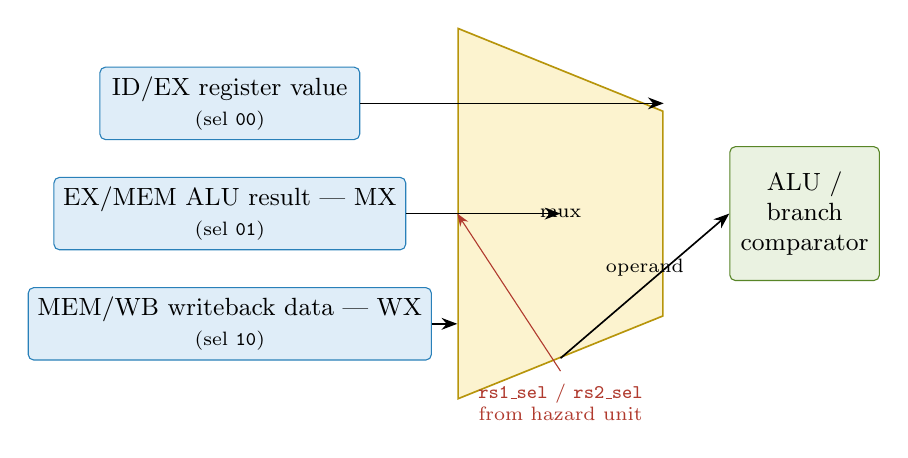
\begin{tikzpicture}[font=\small,
   src/.style={draw=stageline,fill=stagefill,rounded corners=2pt,minimum width=3.3cm,
               minimum height=0.8cm,align=center},
   muxb/.style={draw=regline,fill=regfill,line width=0.6pt},
   alub/.style={draw=auxline,fill=auxfill,rounded corners=2pt,minimum width=1.9cm,
                minimum height=1.7cm,align=center},
   ar/.style={-{Stealth[length=2mm]},line width=0.6pt}]

% three sources
\node[src] (a) at (0, 1.4) {ID/EX register value\\\scriptsize(sel \sig{00})};
\node[src] (b) at (0, 0.0) {EX/MEM ALU result --- MX\\\scriptsize(sel \sig{01})};
\node[src] (c) at (0,-1.4) {MEM/WB writeback data --- WX\\\scriptsize(sel \sig{10})};

% mux (trapezoid)
\node[muxb,trapezium,trapezium angle=68,minimum width=0.6cm,minimum height=2.6cm,
      rotate=-90,anchor=center] (mux) at (4.2,0) {};
\node at (4.2,0) {\rotatebox{0}{\scriptsize mux}};

\draw[ar] (a.east) -- (a.east -| mux.north);
\draw[ar] (b.east) -- (mux.west |- b.east) ;
\draw[ar] (c.east) -- (c.east -| mux.south);

% alu
\node[alub] (alu) at (7.3,0) {ALU\ /\\branch\\comparator};
\draw[ar] (mux.east) -- node[above,font=\scriptsize]{operand} (alu.west);

\node[font=\scriptsize,text=hazline,align=center] at (4.2,-2.4)
   {\sig{rs1\_sel} / \sig{rs2\_sel}\\from hazard unit};
\draw[-{Stealth[length=1.6mm]},hazline] (4.2,-2.0) -- (mux.south);
\end{tikzpicture}
\caption{Per-operand forwarding multiplexer in the Execute stage. Each ALU/comparator
operand is selected from the register-file value, the MX (EX/MEM) bypass, or the WX
(MEM/WB) bypass, under control of the hazard unit's select signals.}
\label{fig:fwd}
\end{figure}

\subsection{Load--use stalls}
Forwarding cannot help when the needed value is produced by a \emph{load}, because a
load's data is not available until the end of the Memory stage --- one cycle too late for
the immediately following instruction in Execute. The hazard unit detects this
\emph{load--use} case (a load in EX whose destination matches a source register being
decoded) and inserts a one-cycle stall: it freezes the PC and the IF/ID register
(de-asserting their write enables) and bubbles the ID/EX register. After the stall, the
dependency has become an ordinary forwarding case and proceeds without further penalty.

\subsection{Write--decode stalls}
Because the register file writes synchronously (WB) while reads are combinational (ID), an
instruction in Decode that reads a register being written in the same cycle by an
instruction in Writeback could observe the stale value. PD5 handles this
\emph{write-to-decode} (WD) dependency conservatively by stalling one cycle when a WB-stage
write targets a register that the Decode-stage instruction reads, guaranteeing the updated
value is read on the following cycle. Load--use and WD stalls share the same stall path
(freeze PC and IF/ID, bubble ID/EX).

\subsection{Control-flow flushes}
The Fetch stage speculatively fetches the sequential successor of every instruction. When
a branch is resolved \emph{taken} in Execute, or when a \sig{jal}/\sig{jalr} reaches
Execute, that speculation is wrong: the instructions already fetched into IF/ID and ID/EX
belong to the not-taken path and must be discarded. The hazard unit asserts the IF/ID and
ID/EX flush signals to squash them (converting them to bubbles as described in
Section~\ref{sec:pipelinereg}), while the correct target address --- computed in Execute
and passed through the writeback/target block --- is loaded into the PC. Flushing is
suppressed while the pipeline is stalling, so the two mechanisms never conflict.

\subsection{Store-data forwarding (WM)}
A final, narrower case arises when a store must write a value that is still in flight ---
for example \sig{lw x1, 0(x2)} immediately followed by \sig{sw x1, 4(x2)}. Here the store's
data operand (\sig{rs2}) equals the destination of the instruction now in Writeback. PD5
resolves this at the top level: when the Memory stage holds a store whose \sig{rs2} index
matches the Writeback destination register (and it is not \sig{x0}), the Writeback data is
substituted for the store data before it reaches memory. The hazard unit exposes a port for
this case but leaves it inactive, since the substitution is performed directly in the
top-level \code{pd5} wiring.

%==============================================================================
\section{Verification Methodology}
\label{sec:verif}
%==============================================================================
\subsection{Toolchain and environment}
The design was developed and verified on a Linux environment driven entirely from
\textbf{bash}. The primary simulator was \textbf{ModelSim --- Intel FPGA Starter Edition},
the simulator bundled with the Intel \textbf{Quartus} Prime toolchain; \textbf{Verilator}
is supported as an alternative open-source simulator. Waveforms were captured as VCD files
and inspected in \textbf{gtkwave} (or the ModelSim GUI) to trace signal behaviour cycle by
cycle. The environment is configured by sourcing \code{env.sh}, which sets the project root
and puts the ModelSim and Verilator executables on the path.

\subsection{Build and run flow}
Simulation is driven by a GNU~Make flow layered over a common include file. The core
commands, issued from a deliverable's \code{verif/scripts} directory, are:

\begin{itemize}[leftmargin=1.4cm]
  \item \code{make compile -C verif/scripts/ VSIM=1} --- compile the design and testbench
    under ModelSim (\code{VERILATOR=1} selects Verilator instead).
  \item \code{make run -C verif/scripts/ VSIM=1 TEST=<name>} --- load
    \code{verif/data/<name>.x} into memory and simulate.
  \item \code{... PATTERN\_CHECK=1} --- compare the design's probe signals against the
    golden \code{<name>.pattern} file; a correct design reports ``Checks passed''.
  \item \code{... PATTERN\_DUMP=1} --- dump the probe signals to \code{<name>.dump} for
    inspection.
  \item \code{make package -C verif/scripts/ VSIM=1 PD=pd5 TEAM=<team>} --- produce the
    submission archive.
\end{itemize}

\subsection{Probes and pattern checking}
Verification is anchored on a set of \emph{probe} signals exposed at well-defined points in
every stage (fetch PC and instruction; decoded fields; register-file reads/writes; ALU
result and branch-taken; memory address/size/data; and writeback destination/data/enable).
The mapping from these probes to the internal signals of \code{pd5} is declared in
\code{design/probes.svh}. During a pattern-check run the harness samples the probes each
cycle and compares them against a golden reference pattern; any mismatch pinpoints the
exact cycle and signal that diverged, giving a precise starting point for waveform
debugging. Appendix~\ref{app:probes} lists the probe signals.

\subsection{Program-termination detection}
Because the benchmarks are self-contained programs, the top-level module watches the
instruction stream for termination. Observing an \sig{ecall} (\hex{00000073}) ends the
simulation immediately. For the function-style synthetic benchmarks, observing a return
(\sig{ret}, \hex{00008067}) marks the program as a simple test, after which simulation ends
once the stack pointer \sig{x2} returns to the top of memory (base~+~\code{MEM\_DEPTH}),
indicating the call has unwound cleanly.

\subsection{Test hierarchy}
PD5 was validated at three levels of granularity, summarised in Table~\ref{tab:tests}.

\begin{table}[h]
\centering
\caption{Verification test hierarchy for PD5.}
\label{tab:tests}
\small
\begin{tabular}{@{}l c p{7.2cm}@{}}
\toprule
\textbf{Level} & \textbf{Count} & \textbf{Purpose} \\
\midrule
Directed pattern tests & 3 & \code{test1}--\code{test3}: baseline datapath correctness via golden patterns. \\
Pipeline micro-tests   & 13 & One test per hazard path (see below): confirm each forwarding, stall, and flush mechanism in isolation. \\
\code{rv32-bmarks} --- instruction & 38 & \code{rv32ui-p-*} RISC-V ISA tests, one per RV32I instruction, exercising every opcode. \\
\code{rv32-bmarks} --- full programs & 10 & Complete C benchmarks compiled to RV32I, exercising realistic instruction mixes and control flow. \\
\bottomrule
\end{tabular}
\end{table}

The thirteen pipeline micro-tests target each hazard mechanism individually:
\code{5-stage-pipeline} (baseline flow), \code{br-taken} (control flush),
\code{load-use-stall} (load--use), \code{wd-stall} (write--decode), the MX bypass tests
(\code{mx-bypass-rs1/rs2-alu} and \code{-brcomp}), the WX bypass tests
(\code{wx-bypass-rs1/rs2-alu} and \code{-brcomp}), and \code{wm-bypass-rs2-mem}
(store-data forwarding). Testing forwarding into both the ALU (\code{-alu}) and the branch
comparator (\code{-brcomp}) confirms that bypassed operands reach both consumers correctly.

The full-program benchmarks are \code{SimpleAdd}, \code{SimpleIf}, \code{Swap},
\code{SwapShift}, \code{SumArray}, \code{BubbleSort}, \code{CheckVowel}, \code{Fibonacci},
\code{fact-short}, and \code{gcd}. During bring-up these were run with waveform capture
enabled; the generated \code{.vcd} and \code{.dump} artefacts (for example
\code{BubbleSort.vcd}, \code{Fibonacci.vcd}, \code{gcd.vcd}) provided the cycle-accurate
traces used to confirm correct pipelined execution.

%==============================================================================
\section{Results}
\label{sec:results}
%==============================================================================
PD5 passes the complete verification suite. Every directed pattern test, every pipeline
micro-test, every RV32UI instruction test, and every full-program benchmark completes with
correct results and no pattern-check mismatches. Table~\ref{tab:results} summarises the
outcome by category.

\begin{table}[h]
\centering
\caption{Verification results by category.}
\label{tab:results}
\small
\begin{tabular}{@{}l c c@{}}
\toprule
\textbf{Category} & \textbf{Tests} & \textbf{Result} \\
\midrule
Directed pattern tests (\code{test1}--\code{test3}) & 3  & \textbf{PASS} \\
Pipeline hazard micro-tests                         & 13 & \textbf{PASS} \\
\code{rv32-bmarks} instruction tests (\code{rv32ui-p-*}) & 38 & \textbf{PASS} \\
\code{rv32-bmarks} full-program benchmarks          & 10 & \textbf{PASS} \\
\midrule
\textbf{Total}                                      & \textbf{64} & \textbf{ALL PASS} \\
\bottomrule
\end{tabular}
\end{table}

Waveform inspection confirmed the intended pipeline behaviour: forwarded operands appear at
the Execute stage in the same cycle they are needed; load--use and write--decode
dependencies each cost exactly one bubble; and taken branches and jumps redirect the PC
with the two mis-fetched instructions cleanly squashed to NOPs. Together these results
demonstrate a functionally correct, hazard-safe RV32I pipeline.

%==============================================================================
\section{Conclusion and Future Work}
\label{sec:conclusion}
%==============================================================================
PD5 delivers a complete five-stage, in-order RV32I RISC-V core in SystemVerilog. Building on
the datapath modules validated in the earlier deliverables, its distinctive contribution is
a correct and efficient hazard-management layer: a two-source forwarding network feeding
both the ALU and the branch comparator, one-cycle stalls for the load--use and
write--decode cases that forwarding cannot cover, single-cycle flushing of mis-fetched
instructions after control-flow changes, and store-data forwarding for back-to-back
load--store pairs. The design was exercised from bash under ModelSim (Intel FPGA / Quartus)
with waveform-level debugging and passes the entire \code{rv32-bmarks} suite alongside the
directed and micro-test batteries.

Several extensions would build naturally on this foundation: consolidating the store-forward
(WM) logic fully inside the hazard unit; adding branch prediction to reduce the control-flow
penalty; supporting the RISC-V M extension (integer multiply/divide) or CSR and exception
handling; and carrying the design through FPGA synthesis in Quartus for timing and resource
analysis.

%==============================================================================
\begin{thebibliography}{9}
%==============================================================================
\bibitem{riscv-isa} A.~Waterman and K.~Asanovi\'c (eds.),
  \emph{The RISC-V Instruction Set Manual, Volume I: Unprivileged ISA}, RISC-V
  International.
\bibitem{ph} D.~A.~Patterson and J.~L.~Hennessy,
  \emph{Computer Organization and Design: The Hardware/Software Interface (RISC-V
  Edition)}, Morgan Kaufmann.
\bibitem{course} EECS 4201 Course Project Repository, York University --- project and
  deliverable README files.
\bibitem{modelsim} Intel Corporation, \emph{ModelSim --- Intel FPGA Edition}, bundled with
  Intel Quartus Prime.
\bibitem{verilator} Veripool, \emph{Verilator} --- open-source Verilog/SystemVerilog
  simulator, \url{https://verilator.org/}.
\bibitem{gtkwave} \emph{GTKWave} waveform viewer, \url{https://gtkwave.sourceforge.net/}.
\end{thebibliography}

%==============================================================================
\appendix
\section{Module and file inventory}
\label{app:files}
%==============================================================================
\begin{table}[h]
\centering
\small
\begin{tabular}{@{}l l@{}}
\toprule
\textbf{File} & \textbf{Role} \\
\midrule
\code{pd5.sv}                  & Top level: instantiates and wires all stages, forwarding, WM store forward. \\
\code{fetch.sv}                & Program counter / instruction fetch. \\
\code{memory.sv}               & Byte-addressable memory (instances: imem, dmem). \\
\code{decode.sv}               & Instruction field extraction. \\
\code{igen.sv}                 & Immediate generator (I/S/B/U/J). \\
\code{control.sv}              & Combinational control decoder. \\
\code{register\_file.sv}       & 32$\times$32-bit register file. \\
\code{execute.sv}              & ALU (Execute stage). \\
\code{branch\_control.sv}      & Branch equal / less-than comparison. \\
\code{writeback.sv}            & Writeback source select and next-PC target. \\
\code{pipeline\_registers.sv}  & IF/ID, ID/EX, EX/MEM, MEM/WB registers with stall/flush. \\
\code{hazard\_unit.sv}         & Forwarding, stall, and flush control. \\
\code{constants.svh}           & Opcodes, \sig{funct3}/\sig{funct7}, and ALU operation codes. \\
\code{probes.svh}              & Verification probe signal mapping. \\
\bottomrule
\end{tabular}
\caption{PD5 source files.}
\end{table}

\section{Debug probe signals}
\label{app:probes}
The probe signals sampled during pattern checking, grouped by stage: \emph{Fetch} --- PC,
instruction. \emph{Decode} --- PC, opcode, \sig{rd}, \sig{funct3}, \sig{rs1}, \sig{rs2},
\sig{funct7}, immediate, shift amount. \emph{Register file} --- write enable/destination/
data and both read addresses and read data. \emph{Execute} --- PC, ALU result, branch
taken. \emph{Memory} --- PC, address, access size, data. \emph{Writeback} --- PC, write
enable, destination, data.

\section{Benchmark inventory}
\label{app:bench}
\textbf{Instruction tests (\code{rv32ui-p-*}, 38):} \sig{add}, \sig{addi}, \sig{and},
\sig{andi}, \sig{auipc}, \sig{beq}, \sig{bge}, \sig{bgeu}, \sig{blt}, \sig{bltu},
\sig{bne}, \sig{jal}, \sig{jalr}, \sig{lb}, \sig{lbu}, \sig{lh}, \sig{lhu}, \sig{lui},
\sig{lw}, \sig{or}, \sig{ori}, \sig{sb}, \sig{sh}, \sig{simple}, \sig{sll}, \sig{slli},
\sig{slt}, \sig{slti}, \sig{sltiu}, \sig{sltu}, \sig{sra}, \sig{srai}, \sig{srl},
\sig{srli}, \sig{sub}, \sig{sw}, \sig{xor}, \sig{xori}.

\medskip
\noindent\textbf{Full-program benchmarks (10):} \code{SimpleAdd}, \code{SimpleIf},
\code{Swap}, \code{SwapShift}, \code{SumArray}, \code{BubbleSort}, \code{CheckVowel},
\code{Fibonacci}, \code{fact-short}, \code{gcd}.

\end{document}
